\documentclass[12pt]{article}
\usepackage{amsmath}
\usepackage{amsfonts} 
\usepackage{amssymb} 
\usepackage{times}
\usepackage{color,hyperref}
  \usepackage{graphicx}
\usepackage{amsthm}
\newtheorem{corollary}{Corollary}
\newtheorem{definition}{Definition}
\newtheorem{result}{Result}
\newtheorem{lemma}{Lemma}
\newtheorem{theorem}{Theorem}
\newtheorem{fact}{Fact}
\hypersetup{colorlinks,breaklinks,
            linkcolor=darkblue,urlcolor=darkred,
            anchorcolor=darkblue,citecolor=darkblue}
\definecolor{darkblue}{rgb}{0.0,0.0,0.75}
\definecolor{darkred}{rgb}{0.75,0.0,0}
\newcommand{\Rcode}[1]{{\texttt{#1}}}
\newcommand{\Rpackage}[1]{\textsf{#1}}
\newcommand{\software}[1]{\textsf{#1}}
\newcommand{\R}{\software{R}}
\newcommand{\fixme}[1]{{\color{red} #1}}
\newcommand{\minfi}{\software{minfi}}


\title{\textbf{Lab 6: Minfi}}
%\author{\\ Jean-Philippe Fortin \quad Kasper D. Hansen }
\author{\\ Jean-Philippe Fortin }
\usepackage{Sweave}
\begin{document}
\maketitle

%%%%%%%%%%%%%%%%% Introduction
\section{Introduction}
The goal of today's tutorial is to present a standard analysis workflow of 450K data with the package \Rpackage{minfi}, incorporating the most recent functions added to the package. \\
\\
We will start from the very beginning by reading input raw data (IDAT files) from an example dataset, and ending with a list of candidate genes for differential methylation. Among others, we will cover quality control assessments, different within-array and between-array normalizations, SNPs removal, sex prediction, differentially methylated positions (DMPs) analysis and bump hunting for differentially methylated regions (DMRs). \\
\\ 
If time permits, we will introduce a complementary visualization tool package, \Rpackage{shinyMethyl}, that allows interactive quality control assessment and principal component analysis (PCA). You can download the package online from shinymethyl.com and try it online.
\subsection*{450k Array design and terminology}
In this section, we introduce briefly the 450K array as well as the terminology used throughout the \Rpackage{minfi} package. 
Each sample is measured on a single array, in two different color channels (red and green). As the name of the platform indicates, each array measures more than 450,000 CpG positions. For each CpG, we have two measurements: a methylated intensity and an unmethylated intensity. Depending on the probe design, the signals are reported in different colors:
\\
\\
For \textbf{Type I} design, both signals are measured in the same color: one probe for the methylated signal and one probe for the unmethylated signal.
\\
\\
For \textbf{Type II} design, only one probe is used. The  \textbf{\textcolor[rgb]{0,0.6,0}{Green}} intensity measures the methylated signal, and the  \textbf{\textcolor[rgb]{0.7,0,0}{Red}} intensity measures the unmethylated signal. 


%%%FIGURE 1
 \begin{figure}
\centering
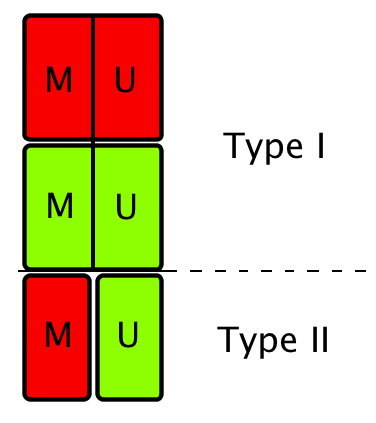
\includegraphics[scale=0.20]{images/designNew.png}
\caption{\textbf{Probe design of the 450k array} For \textbf{Type I} design, both signals are measured in the same color: one probe for the methylated signal and one probe for the unmethylated signal. For \textbf{Type II} design, only one probe is used. The  \textbf{\textcolor[rgb]{0,0.6,0}{Green}} intensity measures the methylated signal, and the  \textbf{\textcolor[rgb]{0.7,0,0}{Red}} intensity measures the unmethylated signal. 
 }
\end{figure}

\subsection*{Some definitions}
Two commonly measures are used to report the methylation levels: Beta values and M values. \\
\\
\textbf{Beta value}: 
\begin{equation*}
\beta = \frac{M}{M + U + 100}
\end{equation*}
where $M$ and $U$ denote the methylated and unmethylated signals respectively. 
\\
\\
\textbf{MValue}:
\begin{equation*}
Mval = \log{\biggl(\frac{M}{U}\biggr)}
\end{equation*}
\\
\\
\textbf{DMP:}  Differentially methylated position: single genomic position that has a different methylated level in two different groups of samples (or conditions)
\\
\\
\textbf{DMR}: Differentially methylated region: when consecutive genomic locations are differentially methylated in the same direction. 
\\
\\
\textbf{Array}: One sample 
\\
\\
\textbf{Slide}: Physical slide containing 12 arrays ($6 \times 2$ grid)
\\
\\
\textbf{Plate:} Physical plate containing at most 8 slides (96 arrays). For this tutorial, we use \textbf{batch} and plate interchangeably. 
\\
\\
%%%% Reading data
\section{Reading Data}
The starting point of \Rpackage{minfi} is reading the .IDAT files with the built-in function \Rcode{read.450k.exp}. Several options are available: the user can specify the sample filenames to be read in along with the directory path, or can specify the directory that contains the files. In the latter case, all the files with the extension .IDAT located in the directory will be loaded into \R{}. The user can also read in a sample sheet, and then use the sample sheet to load the data into a \Rcode{RGChannelSet}. For more information, see the \texttt{minfi} vignette. Here, we will load the dataset containing 6 samples from the \texttt{minfiData} package using the sample sheet provided within the package:
\begin{Schunk}
\begin{Sinput}
> require(minfi)
> require(minfiData)
\end{Sinput}
\end{Schunk}
\begin{Schunk}
\begin{Sinput}
> baseDir <- system.file("extdata",package="minfiData")
> targets <- read.450k.sheet(baseDir)
> targets
> RGSet <- read.450k.exp(base = baseDir, targets = targets)
\end{Sinput}
\end{Schunk}
The class of RGSet is a \Rcode{RGChannelSet} object. This is the initial object of a \minfi{} analysis that contains the raw intensities in the green and red channels. Note that this object contains the intensities of the internal control probes as well. Because we read the data from a data sheet experiment, the phenotype data is also stored in the \Rcode{RGChannelSet} and can be accessed via the accessor command \Rcode{pData}:
\begin{Schunk}
\begin{Sinput}
> phenoData <- pData(RGSet)
> phenoData[,1:6]
\end{Sinput}
\end{Schunk}
The \Rcode{RGChannelSet} stores also a manifest object that contains the probe design information of the array:
\begin{Schunk}
\begin{Sinput}
> manifest <- getManifest(RGSet)
> manifest
> head(getProbeInfo(manifest))
\end{Sinput}
\end{Schunk}
For instance, one can extract the probe names for Type I probes as follows:
\begin{Schunk}
\begin{Sinput}
> typeIProbes <- getProbeInfo(manifest, type = "I")$Name
> head(typeIProbes)
\end{Sinput}
\end{Schunk}
The 450K array contains also 65 SNP probes that do not interrogate methylation. They can be used as control probes to check whether or not samples have been mixed up:
\begin{Schunk}
\begin{Sinput}
> snpProbesI <- getProbeInfo(manifest, type = "SnpI")$Name
> snpProbesII <- getProbeInfo(manifest, type = "SnpII")$Name
> head(snpProbesI)
\end{Sinput}
\end{Schunk}
%%%%%%% Quality control
\section{Quality control}
\minfi{} provides several functions and diagnostic plots to assess quality of the methylation samples. As a starting point, we suggest to look at the function \texttt{detectionP()} which identifies failed positions defined as both the methylated and unmethylated channel reporting background signal levels:
\begin{Schunk}
\begin{Sinput}
> detP <- detectionP(RGSet)
> failed <- detP > 0.01
> head(failed, n=3)
\end{Sinput}
\end{Schunk}
To compute the fraction of failed positions per sample:
\begin{Schunk}
\begin{Sinput}
> colMeans(failed) 
\end{Sinput}
\end{Schunk}
and to compute for instance how many positions failed in $>50\%$ of the samples: 
\begin{Schunk}
\begin{Sinput}
> sum(rowMeans(failed)>0.5)
\end{Sinput}
\end{Schunk}
\subsubsection*{QC plot}
\minfi{} provides a simple quality control plot that uses the log median intensity in both the methylated (M) and unmethylated (U) channels. When plotting these two medians against each other, it has been observed that good samples cluster together, while failed samples tend to separate and have lower median intensities. We need need to convert the \Rcode{RGChannelSet} to an object containing the methylated and unmethylated signals using the function \Rcode{preprocessRaw}. It takes as input a \Rcode{RGChannelSet} and converts the red and green intensities to methylated and unmethylated signals according to the probe design stored in the manifest object, and returns the converted signals in a new object of class \texttt{MethylSet}. Notice that no normalization has been done so far. 
\begin{Schunk}
\begin{Sinput}
> MSet <- preprocessRaw(RGSet) 
> MSet
\end{Sinput}
\end{Schunk}
The accessors \Rcode{getMeth} and \Rcode{getUnmeth} can be used to access the methylated and unmethylated intensities:
\begin{Schunk}
\begin{Sinput}
> head(getMeth(MSet)[,1:3])
> head(getUnmeth(MSet)[,1:3])
\end{Sinput}
\end{Schunk}
We will talk more about the \Rcode{MethylSet} later. The functions \Rcode{getQC} and \Rcode{plotQC} are designed to extract the quality control information from the \Rcode{MethylSet}:
\begin{Schunk}
\begin{Sinput}
> qc <- getQC(MSet)
> head(qc)
> plotQC(qc)
\end{Sinput}
\end{Schunk}
To further explore the quality of the samples, it is useful to look at the Beta value densities of the samples, with the option to color the densities by group:
\begin{Schunk}
\begin{Sinput}
> densityPlot(MSet, sampGroups = phenoData$Sample_Group, main= "Beta", xlab = "Beta")
\end{Sinput}
\end{Schunk}
or density bean plots:
\begin{Schunk}
\begin{Sinput}
> densityBeanPlot(MSet, sampGroups = phenoData$Sample_Group)
\end{Sinput}
\end{Schunk}


Finally, the 450k array contains several internal control probes that can be used to assess the quality control of different sample preparation steps (bisulfite conversion, hybridization, etc.). The values of these control probes are stored in the initial \Rcode{RGChannelSet} and can be plotted by using the function \Rcode{controlStripPlot} and by specifying the control probe type:
\begin{Schunk}
\begin{Sinput}
> controlStripPlot(RGSet, controls="BISULFITE CONVERSION II")
\end{Sinput}
\end{Schunk}
All the plots above can be exported into a pdf file in one step using the function \texttt{qcReport}:
\begin{Schunk}
\begin{Sinput}
> qcReport(RGSet, pdf= "qcReport.pdf")
\end{Sinput}
\end{Schunk}
When the number of samples becomes large, it becomes difficult to assess quality control using the generated plots above.


%%% MethylSet and RatioSet
\section{MethylSet and RatioSet}
As said before, the \Rcode{MethylSet} contains the methylated and unmethylated signals, but no methylation level statistic such as Beta values of M values. We can compute the Beta values or M values from a \Rcode{MethylSet} using  the commands \Rcode{getBeta} and \Rcode{getM}:
\begin{Schunk}
\begin{Sinput}
> getBeta(MSet, type = "Illumina")[1:4,1:3]
> getM(MSet)[1:4,1:3]
\end{Sinput}
\end{Schunk}
Note that the option \texttt{type = "Illumina"} means that a constant of 100 is added in the denominator. Similarly, as seen before, \texttt{getMeth} and \texttt{getUnmeth} return methylated and unmethylated intensities respectively . 
\\
\\
The \Rcode{RatioSet} object class is designed to store Beta values and/or M values instead of the methylated and unmethylated signals. An optional copy number matrix, \Rcode{CN}, which is the sum of the methylated and unmethylated signals, can be also stored. Mapping a \Rcode{MethylSet} to a \Rcode{RatioSet} is irreversible, i.e. one cannot technically retrieve the methylated and unmethylated signals from a \Rcode{RatioSet}.  A \Rcode{RatioSet} can be created with the function \Rcode{ratioConvert}:
\begin{Schunk}
\begin{Sinput}
> ratioSet <- ratioConvert(MSet, what = "both", keepCN = TRUE)
> ratioSet
\end{Sinput}
\end{Schunk}
The functions \Rcode{getBeta}, \Rcode{getM} and \Rcode{getCN} return respectively the Beta value matrix, M value matrix and a the Copy Number matrix. 
%%% Map to Genome
\section{SNPs}
%%% Map to Genome
\section{Map to Genome}
The \Rcode{RatioSet} object is an object containing the final Beta values and M values for further analysis. The function \Rcode{mapToGenome} applied to a \Rcode{RatioSet} object will add genomic coordinates to each probe together with some additional annotation information. The output object is a \Rcode{GenomicRatioSet} (class holding M or/and Beta values together with associated genomic coordinates). It is possible to merge the manifest object with the genomic locations by setting the option \Rcode{mergeManifest} to \Rcode{TRUE}.
\begin{Schunk}
\begin{Sinput}
> gRatioSet <- mapToGenome(ratioSet, mergeManifest = TRUE)
> gRatioSet
> showClass("GenomicRatioSet")
\end{Sinput}
\end{Schunk}
Note that the \texttt{GenomicRatioSet} extends the class \texttt{SummarizedExperiment}. Here are the main accessors functions to access the data:
\begin{Schunk}
\begin{Sinput}
> getBeta(gRatioSet)
> getM(gRatioSet)
> getCN(gRatioSet)
\end{Sinput}
\end{Schunk}
\begin{Schunk}
\begin{Sinput}
> sampleNames <- sampleNames(gRatioSet)
> probeNames <- featureNames(gRatioSet)
> pheno <- pData(gRatioSet)
\end{Sinput}
\end{Schunk}
The accessor \Rcode{rowData} will extract a \Rcode{GenomicRanges} object from the \Rcode{GenomicRatioSet}:
\begin{Schunk}
\begin{Sinput}
> gRanges <- rowData(gRatioSet)
> head(gRanges, n= 3)
\end{Sinput}
\end{Schunk}
To get the full annotation available, one can use the command \Rcode{getAnnotation}:
\begin{Schunk}
\begin{Sinput}
> annotation <- getAnnotation(gRatioSet)
> names(annotation)
\end{Sinput}
\end{Schunk}
%%% Preprocessing and normalization
\section{Preprocessing and normalization}
So far, we have processed the data with no normalization at all. Different normalization procedures are available in \texttt{minfi}. 
\subsection*{preprocessRaw}
As seen before, it converts a \texttt{RGChannelSet} to a \texttt{MethylSet} by converting the Red and Green channels into a matrix of methylated signals and a matrix of unmethylated signals. No normalization is performed. 
\\
\\
Input: \Rcode{RGChannelSet}\\
Output: \Rcode{MethylSet}
%%% preprocessIllumina
\subsection*{preprocessIllumina}
Convert a \texttt{RGChannelSet} to a \texttt{MethylSet} by implementing the preprocessing choices as available in Genome Studio: background subtraction and control normalization. Both of them are optional and turning them off is equivalent to raw preprocessing (\texttt{preprocessRaw}):
\begin{Schunk}
\begin{Sinput}
> MSet.illumina <- preprocessIllumina(RGSet, bg.correct = TRUE,
+                                normalize = "controls")
\end{Sinput}
\end{Schunk}
Input: \Rcode{RGChannelSet}\\
Output: \Rcode{MethylSet}
%%% preprocessSWAN
\subsection*{preprocessSWAN}
Perform Subset-quantile within array normalization (SWAN) [4], a within-array normalization correction for the technical differences between the Type I and Type II array designs. The algorithm matches the Beta-value distributions of the Type I and Type II probes by applying a within-array quantile normalization separately for different subsets of probes (divided by CpG content). The input of SWAN is a \texttt{MethylSet}, and the function returns a \texttt{MethylSet} as well. If an \texttt{RGChannelSet} is provided instead, the function will first call \texttt{preprocessRaw} on the \texttt{RGChannelSet}, and then apply the SWAN normalization. We recommend setting a seed (using \texttt{set.seed}) before using \texttt{preprocessSWAN} to ensure that the normalized intensities will be reproducible. 
\begin{Schunk}
\begin{Sinput}
> MSet.swan <- preprocessSWAN(RGSet)
\end{Sinput}
\end{Schunk}
Input: \Rcode{RGChannelSet} or \Rcode{MethylSet}\\
Output: \Rcode{MethylSet}

%%% PreprocessQuantile
\subsection*{preprocessQuantile}
The function \Rcode{preprocessQuantile()} is a useful one-step command to convert directly a basic \Rcode{RGChannelSet} to a \Rcode{GenomicRatioSet}, i.e. convert red and green intensities to final beta values, M values, copy number estimates and genomic locations. It also implements a between-array normalization called ``Stratified Subset Quantile Normalization". The function has several internal and optional steps available: 
\begin{itemize}
\item[1)] Fix outliers of both the methylated and unmethylated channels (optional)
\item[2)] Remove bad samples using quality control (optional)
\item[3)] Map to the genome using \texttt{mapToGenome}
\item[4)] Perform stratified subset quantile normalization (optional)
\item[5)] Predict the sex if not provided using the function \texttt{getSex} 
\end{itemize}
We have covered all steps mentioned above except the stratified subset quantile normalization (SSQN). What SSQN does is 
\begin{itemize}
\item Perform the quantile normalization on the methylated and unmethylated channels separately
\item The quantile normalization is applied separately on 3 different subsets of probes: autosomal probes, X-chr probes and Y-chr probes. For the X-chr and Y-chr probes, samples are quantile normalized separately by sex.
\item If \texttt{stratified = TRUE}, the subset of autosomal probes is further divided into three subsets: probes mapping to CpG islands, probes mapping to CpG shores, and the rest of the probes. Quantile normalization is then applied separately for each subset of probes
\end{itemize}

\begin{Schunk}
\begin{Sinput}
> gRatioSet.quantile <- preprocessQuantile(RGSet, fixOutliers = TRUE,
+ removeBadSamples = TRUE, badSampleCutoff = 10.5,
+ quantileNormalize = TRUE, stratified = TRUE, 
+ mergeManifest = FALSE, sex = NULL)
\end{Sinput}
\end{Schunk}
Input: \Rcode{RGChannelSet}\\
Output: \Rcode{GenomicRatioSet}
%%% preprocessFunnorm
\subsection*{preprocessFunnorm}
The function \Rcode{preprocessFunnorm()} implements the functional normalization algorithm. Briefly, it uses the internal control probes present on the array to infer the between-array technical variation. It is particularly useful for studies comparing conditions with known large-scale differences, such as cancer/normal studies, or between tissue studies. It has been shown that for such studies, functional normalization outperforms other existing approaches. By default, is uses the first two principal components of the control probes to infer the unwanted variation. One can change the number of principal components via the option \Rcode{nPCs}. Suggested use: 
\begin{Schunk}
\begin{Sinput}
> gRatioSet.funnorm <- preprocessFunnorm(RGSet)
\end{Sinput}
\end{Schunk}
Input: \Rcode{RGChannelSet}\\
Output: \Rcode{GenomicRatioSet}

%%% dmpFinder
\section{dmpFinder: to find differentially methylated positions (DMPs)}
To find differentially methylated positions with respect to a covariate, one can use the function \texttt{dmpFinder}. The phenotype may be categorical (e.g. cancer vs. normal) or continuous (e.g. blood pressure). Let's apply \texttt{dmrFinder} on the genomicRatioSet.quantile that we have created above, with the predicted sex as the phenotype: 
\begin{Schunk}
\begin{Sinput}
> beta <- getBeta(gRatioSet.quantile)
> predictedSex <- pData(gRatioSet.quantile)$predictedSex
> dmp <- dmpFinder(beta, pheno = predictedSex  , type = "categorical")
> head(dmp)
\end{Sinput}
\end{Schunk}
%%% Bumphunter
\section{Bumphunter: to find differentially methylated regions (DMRs)}
The \texttt{bumphunter} function in \texttt{minfi} is a version of the bump hunting algorithm [5] adapted to the 450k array, relying on the \texttt{bumphunter} function implemented in the eponym package \texttt{bumphunter} [6]. \\
\\
Instead of looking for association between a single genomic location and a phenotype of interest, \texttt{bumphunter} looks for association with \textbf{genomic regions}. In the context of the 450k array, the algorithm first defines \textit{clusters} of probes. Clusters are simply groups of probes such that two consecutive probe locations in the cluster are not separated by more than some distance \texttt{mapGap}. To find the differentially methylated regions, the following statistical model is used.
%%%   bump figure 
% \begin{figure}
%\centering
%\includegraphics[scale=0.50]{bump.png}
%\caption{}
%\end{figure}


 \subsection*{Underlying statistical model for bumphunter}
(statistical model described in [6]) We assume that we have data $Y_{ij}$, here Beta-values of M-values, where $i$ represents biological replicate, and $l_j$ represents a genomic location. The basis statistical model is 
\begin{equation*}
Y_{ij} = \beta_0(l_j) + \beta_1(l_j)X_j + \epsilon_{ij}
\end{equation*}
with $i$ representing subject, $l_j$ representing the $j$th location, $X_j$ is the covariate of interest (for example $X_j=1$ for cases and $X_j=0$ otherwise), $\epsilon_{ij}$ is measurement error, $\beta_0(l)$ is a baseline function, and $\beta_1(l)$ is the parameter of interest, which is a function of location. We assume that $\beta_1(l)$ will be equal to zero over most of the genome, and we want to identify segments where $\beta_1 \not = 0$, which we call \textbf{bumps}. 
\\
\\
We want to share information between nearby locations, typically through some form of smoothing. As explained in [[[]], the algorithm can be summarized into the following main steps:
\begin{itemize}
\item[A.] Compute the coefficients $\beta_1(l_j)$ at each genomic location $l_j$.
\item[B.] Optional smoothing of the coefficients $\beta_1(l_j)$ across genomic locations within a cluster of probes
\item[C.] Define a candidate region as a region for which$\beta_1(l_j)$ exceeds a given predefined threshold for all probes within the region
\item[D.] Test for significance of the candidate regions using a permutation scheme 
\end{itemize}
Since the permutation test is expensive, parallel computation is implemented in the \texttt{bumphunter} function. The \texttt{foreach} package allows different parallel ``back-ends" that will distribute the computation across multiple cores in a single machine, or across machines in a cluster. 

\begin{Schunk}
\begin{Sinput}
> pheno <- pData(gRatioSet.quantile)$age
> designMatrix <- model.matrix(~ pheno)
> dmrs <- bumphunter(gRatioSet.quantile, design = designMatrix, cutoff = 0.05, B=1)
> names(dmrs)
> head(dmrs$table, n = 3)
\end{Sinput}
\end{Schunk}

%%% Sex prediction
\section{Sex prediction}

By looking at the median total intensity of the X chromosome-mapped probes, denoted $med(X)$, and the median total intensity of the Y-chromosome-mapped probes, denoted $med(Y)$, one can observe two different clusters of points corresponding to which gender the samples belong to. To predict the gender, \texttt{minfi} separate the points by using a cutoff on $\log_2{med(Y)}-\log_2{med(Y)}$. The default cutoff is $-2$.  Since the algorithm needs to map probes to the X-chr and to the Y-chr, the input of the function \texttt{getSex()} needs to be a \texttt{GenomicMethylSet} or a \texttt{GenomicRatioSet}. 
\begin{Schunk}
\begin{Sinput}
> predictedSex <- getSex(gRatioSet, cutoff = -2)$predictedSex
> head(predictedSex)
\end{Sinput}
\end{Schunk}
To choose the cutoff to separate the two gender clusters, one can plot $med(Y)$ against $med(Y)$ with the function \texttt{plotSex}:
\begin{Schunk}
\begin{Sinput}
> plotSex(getSex(gRatioSet, cutoff = -2))
\end{Sinput}
\end{Schunk}
Furthermore, \texttt{shinyMethyl} has a panel which allow the user to choose interactively the cutoff. 
\\
\\
\textit{Remark}: the function does not handle datasets with only females or only males



\section*{References}
\begin{itemize}
\item[[1]] Hansen, K.D. and Aryee, M.
\emph{minfi: Analyze Illumina's 450k methylation arrays. R package version 1.7.8}
\item[[2]] \emph{shinyMethyl at shinyMethyl.com}
\item[[3]] The Cancer Genome Atlas (TCGA): data portal at https://tcga-data.nci.nih.gov/tcga/
\item[[4]] Maksimovic, J., Gordon, L., Oshlack, A.
\emph{SWAN: subset quantile Within-Array Normalization for Illumina Infinium HumanMethylation450 BeadChips}
Genome Biology, 13(6) R44, 2012
\item[[5]] Jaffe, A. E, Murakami, P. Lee, H. Leek, J.T., Fallin, M.D., Feinberg, A.P., Irizarry, R. 
\emph{Bump hunting to identify differentially methylated regions in epidemiology studies}
International Journal of Epidemiology, 41(1): 200-209, 2012
\item[[6]] Irizarry, A.R., Aryee, M., Corrada Bravo, H., Hansen, K.D., Jaffee, H.A
\emph{bumphunter: Bump Hunter, R package version 1.1.10}
\end{itemize}


\section{Exercises}
\begin{itemize}
\item[1)] Before processing a RGChannelSet further, coudl you remove the probes which failed more than $50\%$ of the samples in the example dataset?
\item[2)] For the top loci that we found differentially methylated for the predicted sex, could you tell if those loci are mostly mapped to the X and Y chromosomes? 
\item[3)] It is known that the Beta-value distribution of the Type I probes is different from the Beta value distribution of the Type II probes. Can you verify this with by plotting the Beta-value distribution density for each type separately?  
\end{itemize}

%%%FIGURE 1
 \begin{figure}
\centering
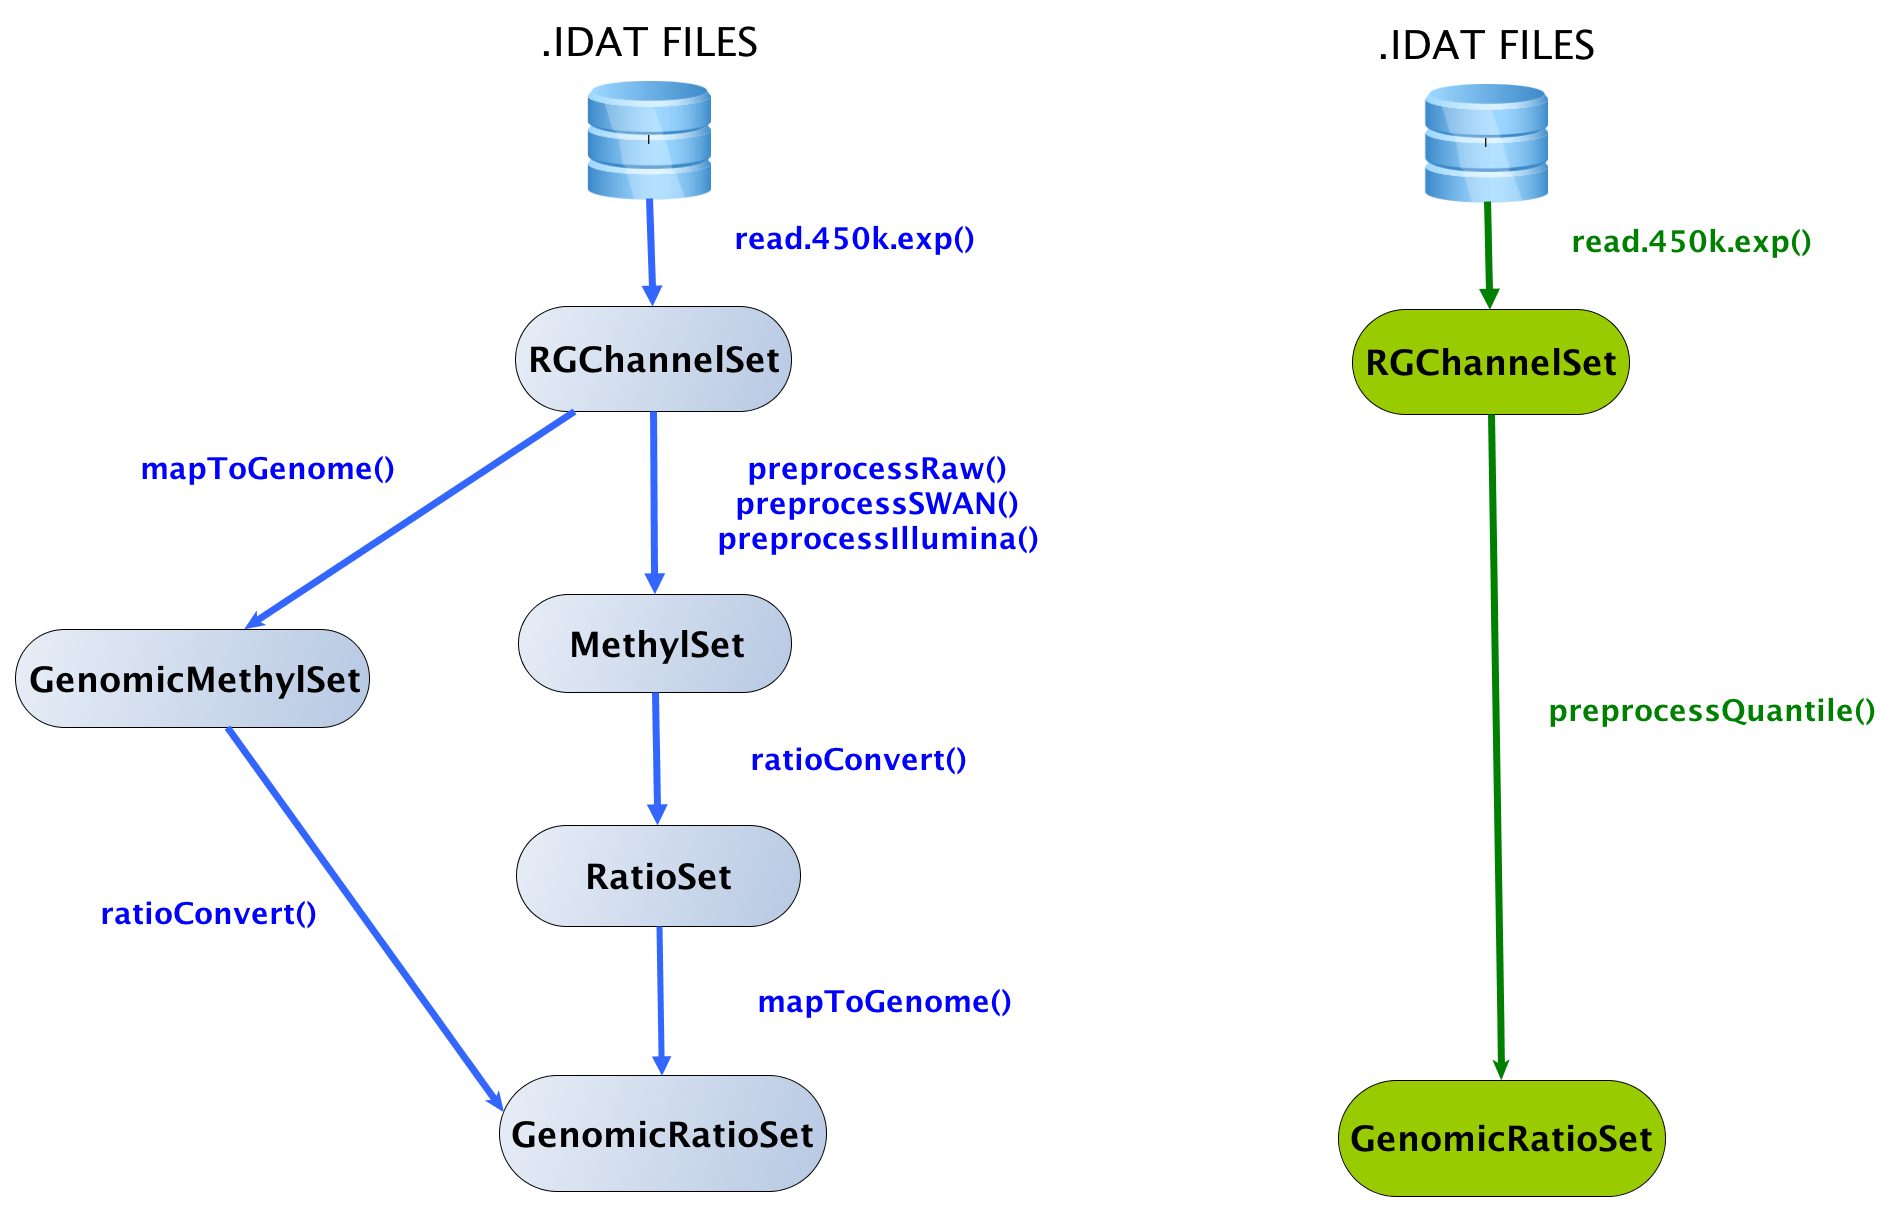
\includegraphics[scale=0.35]{images/flowChart3.png}
\caption{Flow chart of the \texttt{minfi}'s functions}
\end{figure}




%%% Note: include a link to the GenomicRanges package for information about how to handle such objects
\end{document}
